\chapter{One Stage Detector}
After getting stuck for trying to develop a solution that would first do object detection, and then afterward classify the segmented areas separately, it was decided to try a different approach. The one stage detector  \textit{You Only Look Once} method was tried to great success. This chapter will describe how it works, sections \ref{sec:yolo} \ref{sec:mAP}, how the models were created and trained, section \ref{sec:turi}, and then an evaluation of the resulting models in section \ref{sec:turiResults}.

There are other methods of doing object detection and classification, such as \textit{Mask R-CNN} and \textit{Faster R-CNN}, however, they are outside of the scope of this project.
\section{YOLO}
\label{sec:yolo}
YOLO, or You Only Look Once, is a one stage detector approach to object detection and
 recognition \cite{YOLO1}. It takes an image and predicts both bounding boxes and the probabilities of the classes being within these bounding boxes in one run, hence its name. It was designed to be fast and usable in real-time scenarios. Since YOLO sees the entire image during training and testing, it receives contextual information about the classes and reduces error with matching background patches for objects. 
 
 The architecture for \textit{YOLO} consist mainly as a convolutional neural network, with 24 convolutional layers and two fully connected layers. There was also a smaller neural network trained called \textit{Fast YOLO} trained which were only 9 layers which was designed to create an even faster system for object detection. 
 
 The system first divides the input image into an  $S \times S$  grid, where each cell predicts $B$ amount of bounding boxes respectively confidence scores for the boxes. Each bounding box prediction consists of 5 separate predictions: the \textit{x, y} coordinates, represented as their position relative to the the grid cell, width and height relative to the entire image and a confidence value. The confidence values are there to reflect how certain the model is that there exists an object within the box, i.e. ideally, confidence should be zero when no object, and the intersection over union between ground truth and the predicted box if there is. Each grid cell also predicts $C$ probabilities for each class, conditioned that there's an object within the boxes. 
 
 Intersection over union, also known as the Jaccard index, is a way of measuring similarity between sets. It can be written as 
 \[
IOU(A,B) =  \frac{|A\cap B |}{|A\cup B|} =\frac{|A\cap B|}{|A| + |B| - |A \cap B|}
, \quad 0\leq IOU(A,B) \leq 1
 \]
 if $A,B$ are two finite sets. If the two sets are equal, then \[ IOU(A,A) =  \frac{|A\cap A |}{|A\cup A|} = \frac{|A\cap A|}{|A| + |A| - |A \cap A|}  = \frac{|A|}{|A|} = 1 \]
 
 When testing, these scores are then combined to give the class specific confidence values for each of the boxes, thus it receives both the confidence of the class being in the box, and how well the box fits the object. Figure \ref{fig:YOLO_stages} summarizes the flow in YOLO. 
\begin{figure}[hbtp]
\begin{center}
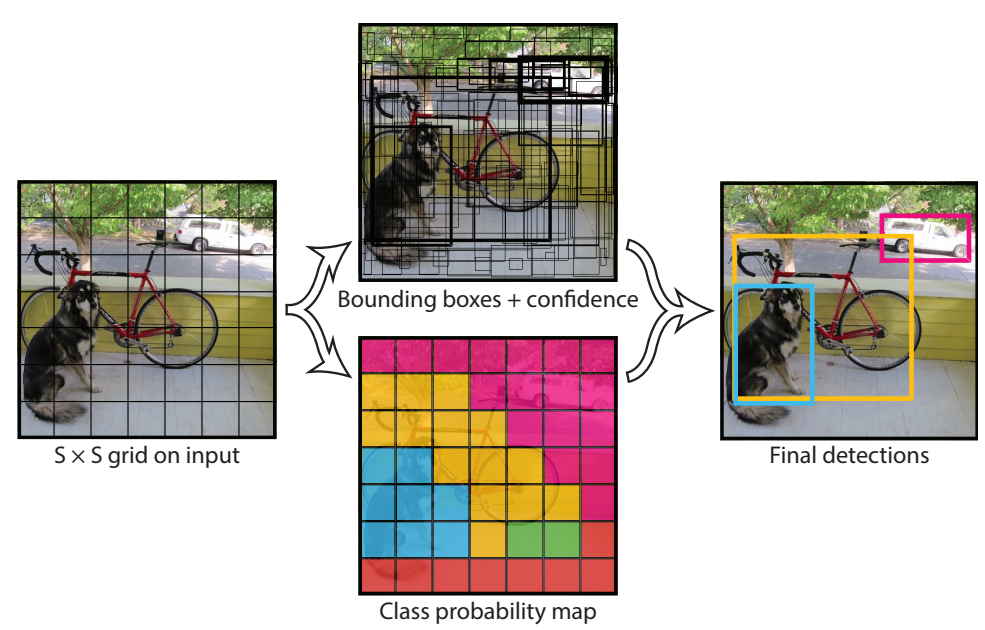
\includegraphics[width = 0.75\textwidth]{./Images/YOLO_stages.PNG} 
\caption{The stages of YOLO. First dives into $S \times S$ grid. Separately predicts bounding boxes with respective confidence, as well as class probability. Then, combines the two to form the final predictions. Image taken from \cite{YOLO1}.}
\label{fig:YOLO_stages}
\end{center}
\end{figure}

Comparisons done by the team working on \textit{YOLO} found that, compared to other real-time systems at the time, both \textit{Fast YOLO} and \textit{YOLO} outperformed them all with \textit{Fast YOLO} being the fastest, but \textit{YOLO} being more accurate on the \textit{PASCAL VOC} data sets \cite{PASCAL}.

Throughout the years Redmon et al. has been working on updating the design pattern of the 
YOLO network. First in 2016 when they introduced \textit{YOLOv2} and then April 2018 with \textit{YOLOv3} \cite{YOLO2}\cite{YOLO3}. \textit{YOLOv2} added a few concepts to the system to make it even more fast and accurate than the earlier iteration. It removed the fully connected layers and it was now possible to train on several different input image resolutions and it could now also predict many more bounding boxes than its predecessor. \textit{YOLOv3} added some changes which improved its ability to detect small objects, with the trade off of having a bit worse performance when finding larger sized objects.  

\section{Mean Average Precision}
\label{sec:mAP}
There is quite a difference when it comes to evaluating a model that does object detection,  compared to normal image classification. When doing the latter, accuracy tells you how often the model makes the correct prediction. However, with object detection it is done differently. The common metric is \textit{mean Average Precision} (mAP).  This metric makes use of the previously discussed \textit{IoU} (Intersection over Union). The IoU and the classification determines if the prediction is deemed correct. The classification obviously has to be the same as the ground truth, and the IoU has to be over a set threshold, these are known as true positives. A predicted box that does not pass the threshold is known as a false positive. If there are more than one prediction that passes the threshold, only one will get seen as a true positive, and the other as false positive. When a prediction was not made for a ground truth box, it is called a false negative \cite{turiAdvanced}.

From the false positives, true positives, and the false negatives, one can calculate recall as well as precision scores \cite{rafaelpadilla}.  Precision is how good the model is to identify only the relevant data, and can be written as
\[ \texttt{precision} = \frac{\texttt{True Positives}}{\texttt{True Positives + False positives }}\]
Recall is how good the model is to find all the relevant data, and is written as 
\[ \texttt{recall} = \frac{\texttt{True Positives}}{\texttt{True Positives +False Negatives }}\]

 When a classification is made you also get a confidence value. One only calls it a prediction if the predictions confidence passes a set threshold. However, if one calculates the recall and precision for all possible thresholds, a Recall x Precision curve can be made. From this curve, one gets the mAP by taking the area under the curve.

There are different standards when calculating the mAP. The PASCAL VOC Challenge uses a mean average precision with a static threshold of 50\%
 \cite{PASCAL}. This is commonly called \textit{mean\_average\_precision\_50}. Another common standard is the one used by COCO  \cite{COCO}. This one calculates the mAP at IoU threshold from 50\%  to 95\%, with increments of 5\% every iteration, and averages them all together. This is quite strangely known as just \textit{mean\_average\_precision}. The latter mentioned method is the one this report will use for evaluation, since it puts more value on localization than the PASCAL VOC method.

\section{Turi Create}
\label{sec:turi}
%Write about the testing an implementation of Turi
Apple has a licenced toolkit for development of custom machine learning models called Turi Create \cite{turiCreate}. This was created to help developers easily implement their own ideas into an app. It includes a methods object detection.

In this project, the object detection method included in Turi Create was tested. First, one
 has to create ground truth data for every image that was trained and tested on. This was
 done using Simple Image Annotator \cite{simpleImage}, where one has to draw bounding
  boxes for the objects in the images and label them; the data output is in the \textit{.csv} format.  Turi Create uses a different format for annotations called \textit{.sframe},
  however, they provide a simple Python script which automatically does the conversion. 

Turi then trains a model using a re-implementation of the TinyYOLO network. It also utilizes transfer learning by starting with an image classifier that has been trained on the imageNet dataset and then does \textit{end-to-end finetuning} to change the network to a \textit{one-stage detector}.

Several models were trained, with different amount of training data, to evaluate how many
 were needed to get a decent result. The Turi website states that at least 30 samples of
each class is needed to generate a good enough model. Hence, we tested for even lower
samples, as well as much more. Lowest amount of training images were around 50, and
highest  were around 1000. The \textit{mean average precision} was measured for each model using 200 testing images, and then plotted to create a graph showing how it
 changed, depending on the amount of training data was used. The results can be seen in section \ref{sec:turiResults}. The best performing model was then to be used in the application.

The code in appendix D.1. shows how the model was created using Turi in python.

The results could also be further inspected by drawing the newly predicted bounding boxes on top of the original image, from this one can visualize how the model actually performed. This was done using code in appendix D.2. Some of the resulting images from different models can be seen in section \ref{sec:turiResults}. 


\subsection{Importing model to application}
After training and evaluating that the model lives up to a standard worth including in this
 project, it was converted to the \textit{.mlmodel} format used in Swift. When inputting a frame from the
application into the model, the model outputs a multi array containing an array for each
  \textit{object} found. These predictions have not been \textit{non-max suppressed}, since that functionality is lost during the conversion from the model used in python, to the .mlmodel format. Thus, it has to be reimplemented in the application itself. 
  A non-max supression threshold of $0.5$ was used as it is considered a traditional standard \cite{nms}. The code in appendix D.3. shows how non-max suppression was implemented. 


\section{Results from doing object detection with Turi}
\label{sec:turiResults}
Because of the vast amount of possible use cases it was decided to scale the objective down. The model was trained only on a few floor backgrounds. 

The mean average precision from the different models that were trained were observed and can be read in table \ref{table:mAP}. These values were plotted, resulting in the graph shown in figure \ref{fig:mAPResult}.


\begin{table}[h]
\centering
\begin{tabular}{ |c|c|c| } 
 \hline
 Amount of training images & Percentage of total amount & mean\_average\_precision  \\ 
 \hline
 $\approx 50$& 5\% & 0.17064 \\
 \hline
 $\approx 100$& 10\% & 0.30188 \\
\hline
  $\approx 140$& 15\% &  0.30342 \\
 \hline
 $\approx 185$& 20\% & 0.39269 \\
 \hline
$\approx 280$ &  30\% & 0.41588 \\
 \hline
 $\approx 370$& 40\% & 0.40595 \\
 \hline
 $\approx 415$& 45\% & 0.49917 \\
 \hline
 $\approx 450$& 50\% & 0.47397 \\
\hline
$\approx 570$ & 60\% & 0.50454 \\
\hline
 $\approx 700$& 75\% & 0.54433 \\
 \hline
$926$ & 100\% & 0.57618 \\
 \hline
\end{tabular}
\caption{Mean average precision depending on the amount of training data used.}
\label{table:mAP}
\end{table}

\begin{figure}[h]
\begin{center}
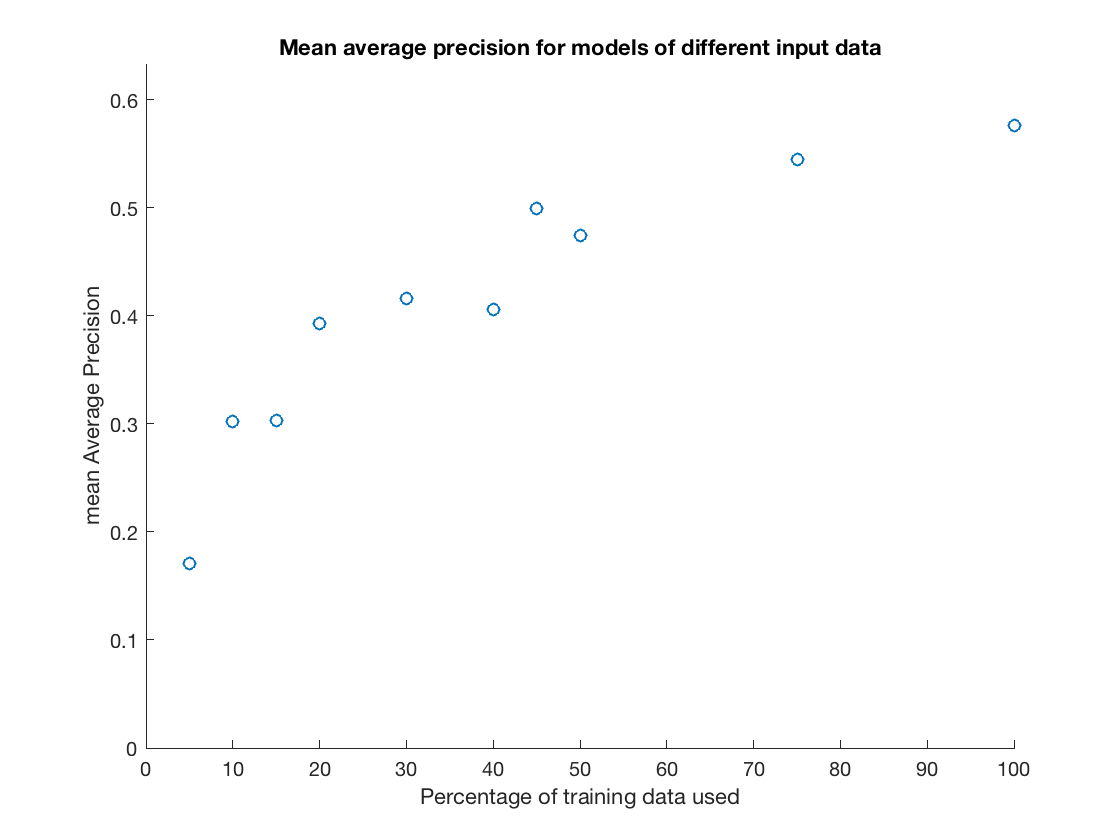
\includegraphics[width = 0.9\textwidth]{./Images/mapPlot.png}
\caption{Mean Average Precision from table \ref{table:mAP} plotted against the amount of training data used. 100\% corresponds to 926 images.}
\label{fig:mAPResult}
\end{center}
\end{figure}

\begin{figure}[h]
\begin{center}
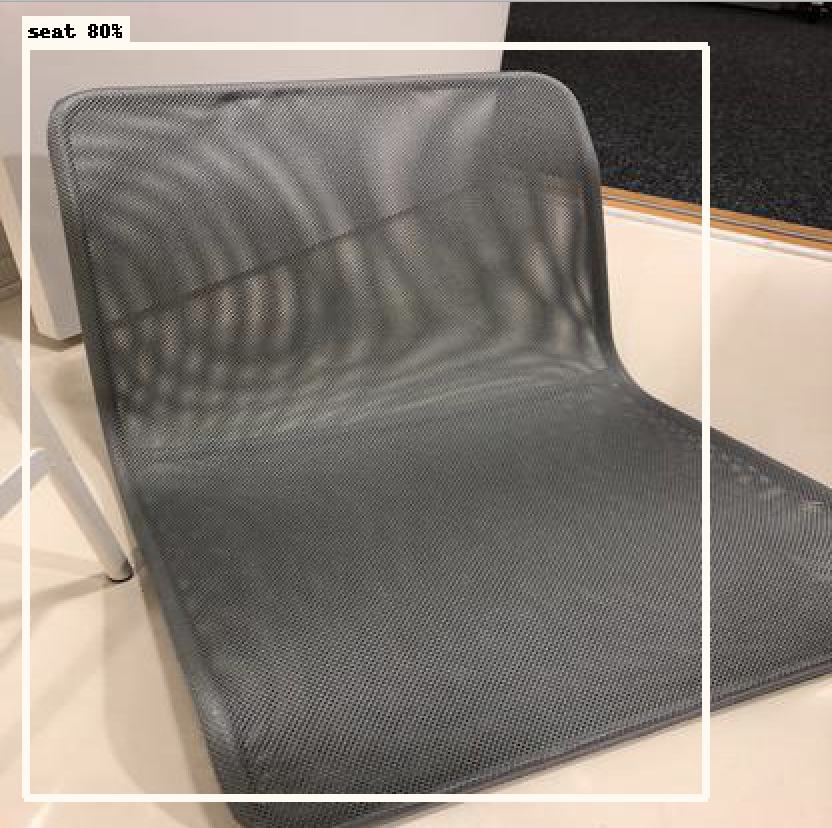
\includegraphics[width = 0.3\textwidth, height = 0.3\textwidth]{./Images/turi100-1.png}
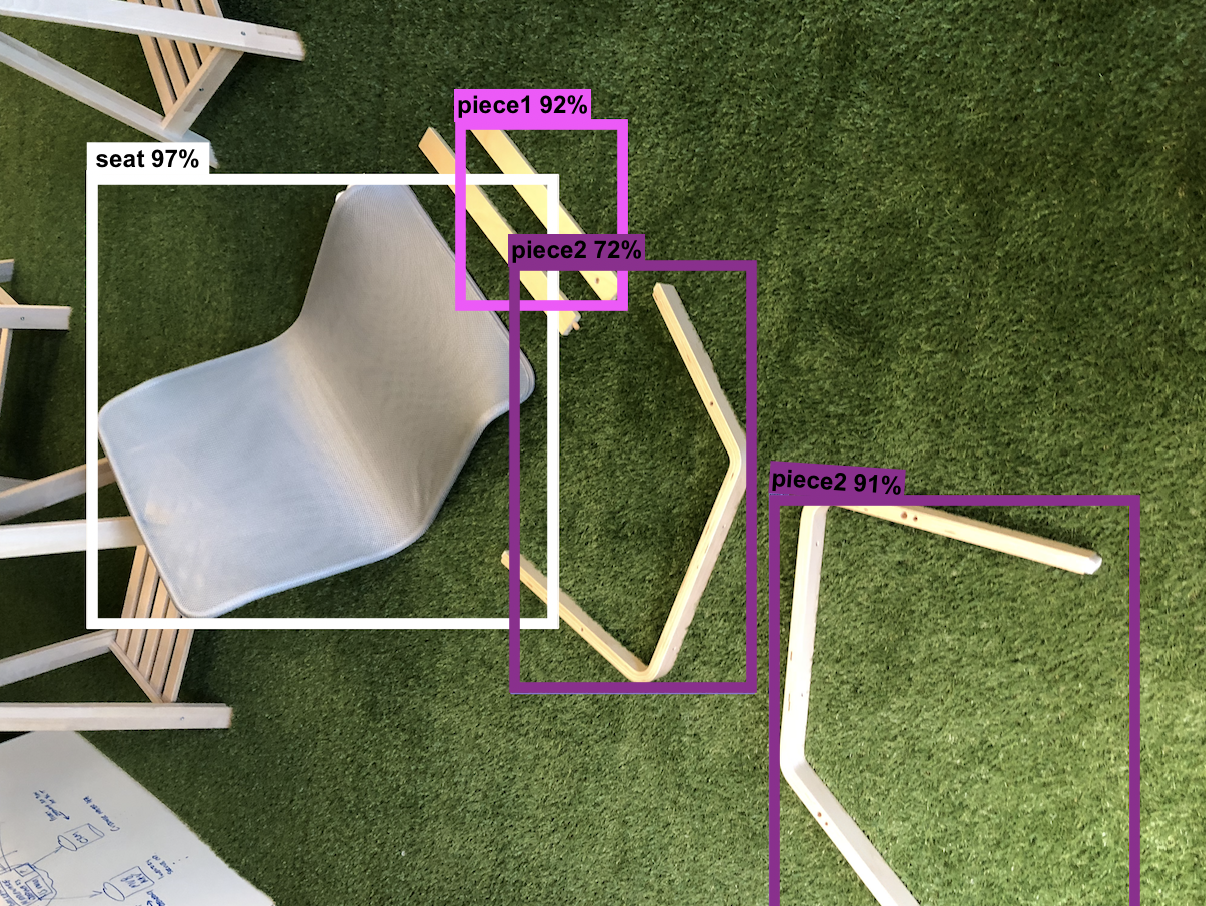
\includegraphics[width = 0.3\textwidth, height = 0.3\textwidth]{./Images/turi100-2.png}
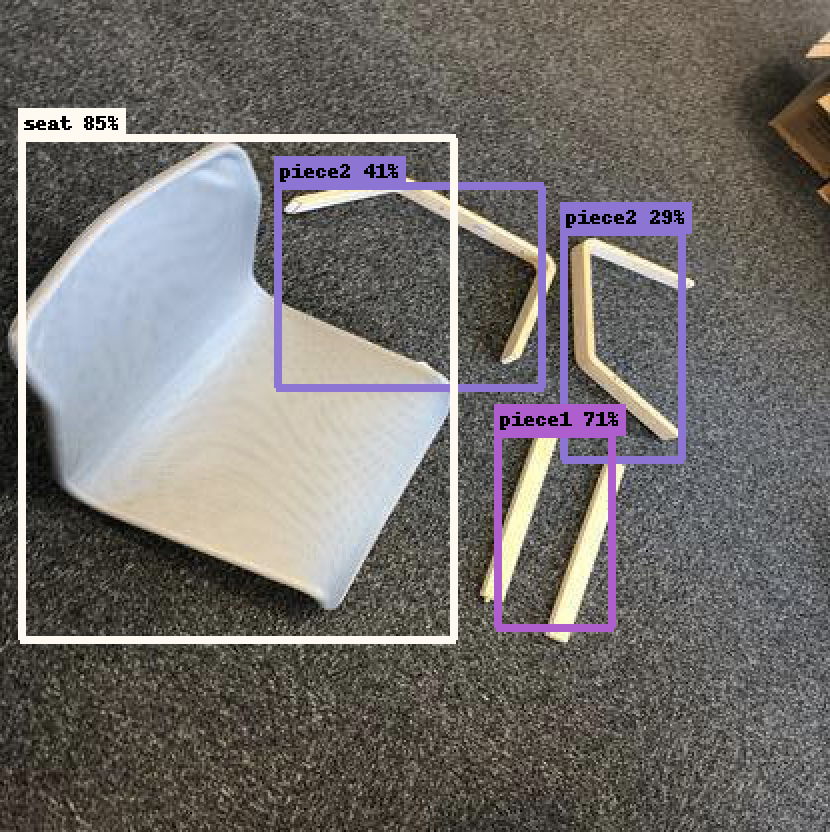
\includegraphics[width = 0.3\textwidth, height = 0.3\textwidth]{./Images/turi100-3.png}
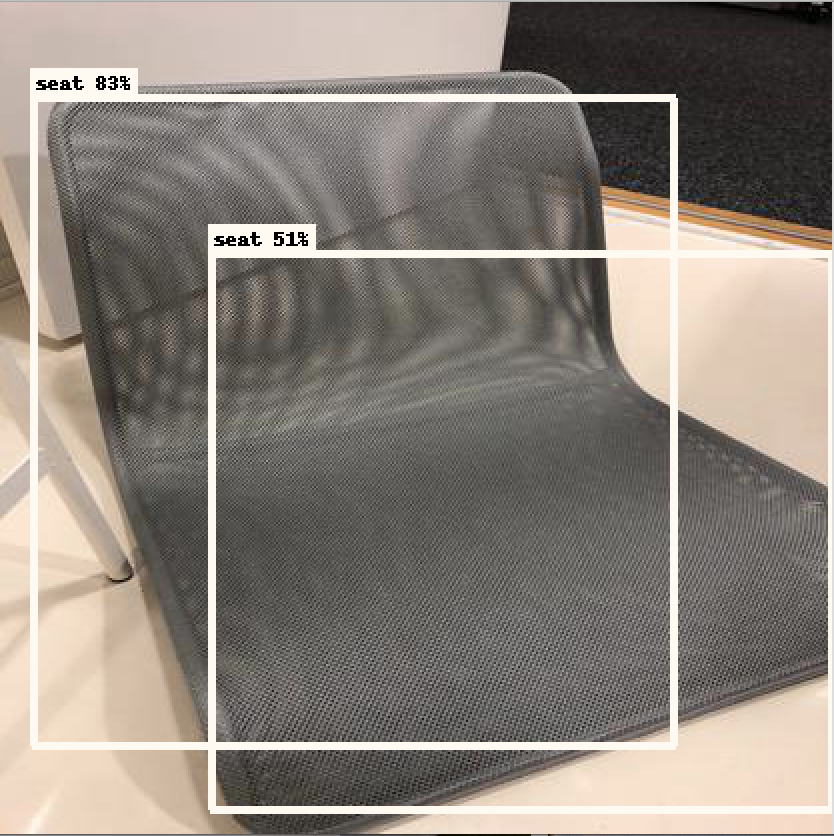
\includegraphics[width = 0.3\textwidth, height = 0.3\textwidth]{./Images/turi015-1.png}
\includegraphics[width = 0.3\textwidth, height = 0.3\textwidth]{./Images/turi015-2.png}
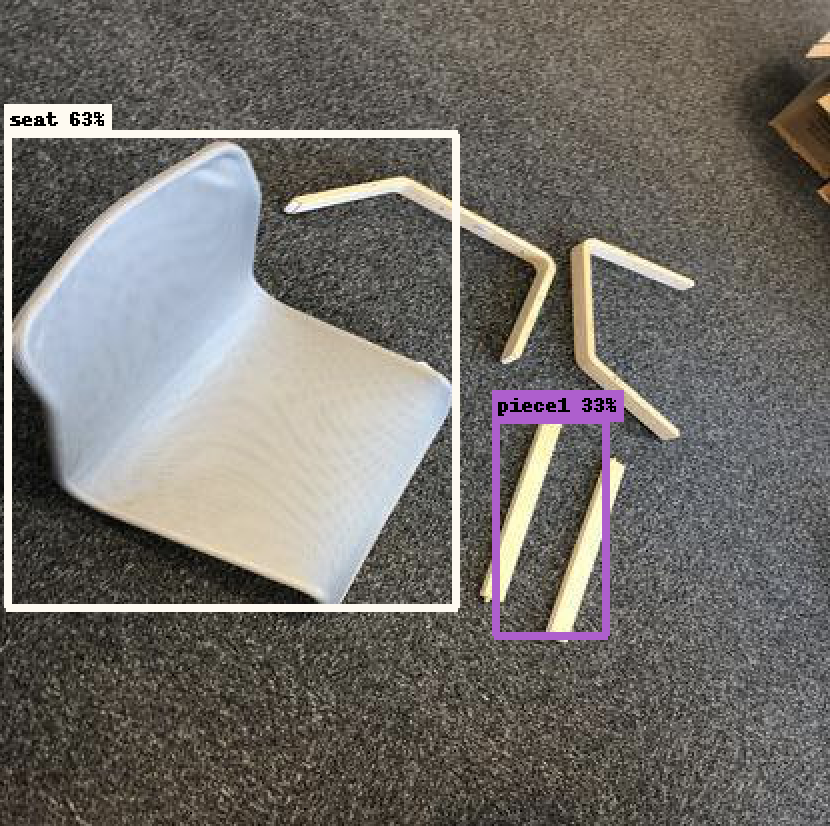
\includegraphics[width = 0.3\textwidth, height = 0.3\textwidth]{./Images/turi015-3.png}
\caption{Images showing how the same three images were classified differently using different models. The top row is classified using the model that was trained on all of the training set. The bottom row shows the images that were trained on only $ 15 \% $ of the training set. }
\label{fig:mAPExamples}
\end{center}
\end{figure}


When training on different amount of data it can appear as if more data gives a worse
result sometimes. That can be explained in two ways. The first explanation is that when
training the models the data was randomly split from the full training data set. That 
means that sometimes there can be more "good" data and sometimes less in the set.
Some images have lots of objects in them and others have fewer. Thus, if you have a
data set with images with lots of objects in them it will likely give better results.
An important thing to mention however is that for the model to perform well it also needs
areas in the image of no object.

The other explanation is that when training, the most optimal model for that data set is
not always, if ever, returned. Take into account early stopping for example.
Sometimes the early stopping can happen on a good place and sometimes it could have
given a better result if the training session would have kept going for a little bit. We did not have a way to use an evaluation set during training, and as such, could not receive training and validation curves. Hence, we can not know how if we trained for too long or too little.

The curve from the tests, fig. \ref{fig:mAPResult}, shows no sign of saturation yet, thus even more data would
surely improve the performance. The reason for not testing with more data is because
of the difficulty of gathering more data (taking photos in different environments and 
adding ground truth data) and the time it took for training.
As of now, the time for training with 926 images on a MacBook Pro 15 inch 2017 with a 2,8 GHz
Intel Core i7 processor is over 24 hours. With half the amount it takes about 17 hours. We would have trained with a GPU, however, it was at the time of training not supported on our hardware.\\

From the graph there is a small plateau between 185 to 370 images. Around that
performance (0.4 mAP) is a sort of minimum for the model to perform well.
For our 6 classes that would correlate to needing around 30-60 images per class.

From the plot in figure \ref{fig:mAPResult} one can see a sharp ascension up until around  20\% of the training set, or 185 images, were used to train the model. This corresponds to roughly 30 images per class. Afterwards, it starts to even out. Hence, the claim that at least 30 images are need to train a somewhat decent model is correct. However, as seen, more data usually generates even better result.

\newpage